\documentclass[../../Main/Main.tex]{subfiles}

\begin{document}

\chapter{Landau theory of phase transition for homogeneous systems}

\section{Introduction to Landau theory}

Landau theory is a phenomenological mean field theory of phase transitions  that aims at describing the occurence of phase transitions in a unitary framework (no spatial variation of the order parameter). Landau theory is based on some assumptions, which we now introduce:
\begin{enumerate}
\item Existence of an uniform order parameter \( \eta   \). Remember the definition of the order parameter:
\begin{equation*}
  \eta   = \begin{cases}
    0 & T \ge \bar{T} \text{ (disordered phase)}\\
    \neq 0 & T < \bar{T}  \text{ (ordered phase)}
\end{cases}
\end{equation*}
Well known examples are
\begin{equation*}
  \begin{cases}
   \eta \rightarrow m \\
  \eta  \rightarrow \rho _L - \rho _G
  \end{cases}
\end{equation*}

\item There exists a function \( \mathcal{L} \)  called Landau free energy\footnote{To be more precise,  \( \mathcal{L} \) is the Landau free energy density; the "real" Landau free energy should be  \( L = V \mathcal{L}  \).}, which is an analytic function of the coupling constants \( \{ K_i\} \) of the system and of the order parameter \( \eta  \):
\begin{equation*}
  \mathcal{L} = \mathcal{L} (\{K_i\},\eta )
\end{equation*}

\item The form of \( \mathcal{L} \) must satisfy the underlying symmetry of the system.
\item The equilibrium states of the system are the global minima of \( \mathcal{L} \) with respect to  \( \eta  \).

\end{enumerate}

We also assume that the thermodynamic properties of the system can be obtained by differentiating \( \mathcal{L} \), just like we can do with thermodynamic potentials\footnote{Strictly speaking, Landau free energy is not really a thermodynamic potential: the correct interpretation of \( \mathcal{L} \) is that it is a coarse grained free energy (not the exact one).}.

Note also that the general formulation of the Landau theory does not depend on the dimensionality of the system (although we will see that once a system has been chosen some details can depend on it).

\begin{remark}
Since \( \mathcal{L} \) is analytic it can be formally expanded in power of \( \eta  \), for \( \eta \sim 0 \).
\begin{empheq}[box=\myyellowbox]{equation}
  \mathcal{L} (\eta ) \approx a_0 + a_1 \eta + a_2 \eta ^2 + a_3 \eta ^3 + \dots
\end{empheq}
\end{remark}

\section{Landau theory for the Ising model}
To make things more clear, let us now consider the Ising model without any external field and see how we can determine the form of \( \mathcal{L} \) from the general assumptions we have introduced. In this case \( \eta  \) is a scalar (magnetization).

\subsection{Costruction of \( \pmb{\mathcal{L} } \) }
First of all, since the equilibrium configurations of the system must be minima of \( \mathcal{L} \) :
\begin{equation*}
  \pdv{\mathcal{L}}{\eta } = a_1 + 2 a _2 \eta + 3 a _3 \eta ^2 + \dots = 0
\end{equation*}
where we have chosen to stop the expansion at the three order. Now, since this equation must hold for all \( T \) and for \( T > \bar{T}  \) \footnote{For \( T > \bar{T}  \) (critical point) we expect a paramagnetic phase.} we have \( \eta =0 \), we see that \( a_1=0 \).

Considering now the constraint on the symmetries of the system, in absence of phase transitions for finite systems we have seen that the Ising model is invariant under parity (\( \mathbb{Z}^2 \) symmetry), i.e. its Hamiltonian is simultaneously even in \( H \) and \( \{S_i\} \):
\begin{equation*}
  \mathcal{H} (H, \{ S_i \}  ) =   \mathcal{H} (-H, \{ -S_i \}  )
\end{equation*}
Thus, in absence of external fields (\( H=0 \)) the Hamiltonian of the Ising model is even; this means that also \( \mathcal{L} \)  must be invariant under parity, namely an even function of \( \eta  \):
\begin{equation*}
  \mathcal{L} (-\eta ) =   \mathcal{L} (\eta )
\end{equation*}
Therefore all the odd terms of the expansion are null:
\begin{equation*}
  a_{2k+1} = 0 \quad \forall k  \in \mathbb{N}
\end{equation*}

Finally, since we have assumed that \( \mathcal{L} \) is an analytic function of  \( \eta  \) then its expansion cannot contain terms proportional to \( \abs{\eta }  \).


In conclusion, the minimal expression for \( \mathcal{L}(\eta ) \) that describes the equilibrium phase diagram of an Ising-like system is:
\begin{empheq}[box=\myyellowbox]{equation}
  \mathcal{L} (\eta ) \simeq a_0 (J,T) + a_2 (J,T) \eta  ^2 + a_4  (J,T) \eta  ^4 + O(\eta ^6)
\end{empheq}
where the coefficients of the expansion \( a_0,a_2,a_4,\dots \) are functions of the physical parameters, \( J \) and \( T \).  However,  \( \mathcal{L} \) can be further simplified and we can also explicitly show its dependence on the temperature.
In fact, first of all we can note that  \( a_0 \) is the value of \( \mathcal{L} \) in the paramagnetic state (when \( T> \bar{T}  \), \( \eta =0 \)):
\begin{equation*}
  \mathcal{L} (\eta =0) = a_0
\end{equation*}
and so for simplicity we can set \( a_0 = 0 \) (it's just a constant shift in the energy, what matters is the free-energy difference).


Moreover, in order to have \( \eta = \bar{\eta } \neq 0 < \infty   \) for \( T < \bar{T} \) (thermodynamic stability) we should impose that the coefficient of the highest power of \( \eta  \) is always positive. In this case:
\begin{equation*}
  a_4 (J,T)>0
\end{equation*}
Indeed if this condition is violated \( \mathcal{L} \) reaches it s absolute minimum for \( \eta  \rightarrow \pm \infty   \), which makes no sense physically! The Landau free energy results
\begin{equation}
    \mathcal{L} (\eta ) \simeq  a_2 \eta  ^2 + a_4  \eta  ^4, \quad \text{with } a_4>0
\end{equation}

Finally, fixing \( J \) and expanding the coefficients \( a_2 \) and \( a_4 \) as a function of the reduced temperature \( t \equiv \frac{T - \bar{T} }{\bar{T} } \) (in \( T \) near \( \bar{T}  \)), we obtain
\begin{equation*}
    a_2  \sim  a_2^0 +    \frac{T - \bar{T} }{\bar{T} } \frac{a}{2} + \dots, \qquad  a_4  \sim \frac{b}{4} + \dots
\end{equation*}
in the expansion of \( a_4 \) we have neglected any explicit dependence on \( T - \bar{T}  \) because as we will see it will not dominate the behaviour of the thermodynamics near \( \bar{T}  \). Moreover, by choosing \( a_2^0 = 0\) the sign of \( a_2 \) is determined by the one of \( t \).
In particular, at \( T = \bar{T}  \), one has \( a_2 =0 \).

We finally have that the form of the Landau free energy for the Ising model is given by:
\begin{empheq}[box=\myyellowbox]{equation}
    \mathcal{L} = \mathcolorbox{green!20}{\frac{a}{2}} t  \eta ^2 + \frac{b}{4} \eta ^4 + O ( \eta ^6)
\end{empheq}

\begin{remark}
Does not matter the coefficient in green in front, so in the next part of the course we will change it. If it is written in this way we have always \( a>0 \). We have also \( b>0 \).
\end{remark}

Note that, in presence of an external magnetic field \( h \), one should consider the Legendre transform of \( \mathcal{L} \) obtaining its Gibbs version:

\begin{equation}
  \mathcal{L}_G =  \frac{a}{2} t \eta ^2 + \frac{b}{4} \eta ^4 - h \eta
\end{equation}
we have inserted a field coupled with the order parameter.


\subsection{Equilibrium phases}
Let us now see what does the Landau theory for the Ising model predict. First of all, in the absence of external fields we have that the equilibrium states are determined by:
\begin{equation}
  \pdv{\mathcal{L}}{\eta } = 0 \quad \Rightarrow  a t \eta + b \eta ^3 = \eta (at+b \eta ^2)= 0
\end{equation}
Hence, the minima are
\begin{equation}
  \bar{\eta } =
  \begin{cases}
   0 & t>0 \,(\text{i.e. } T > \bar{T}) \\
   \pm \sqrt{\frac{-at}{b}} & t<0 \,(\text{i.e. } T < \bar{T})
  \end{cases}
\end{equation}
and at \( T= \bar{T}  \)  the 3 solutions coincide!

Let us consider the two different cases:
\begin{itemize}
\item Case \( t>0 \) (\( T> \bar{T}  \)):  the only global minimum of \( \mathcal{L} \) is the solution \( \bar{\eta }=0  \). The second derivative of \( \mathcal{L} \) with respect to \( \eta  \) is
\begin{equation*}
  \pdv[2]{\mathcal{L}}{\eta } = a t + 3 b \eta ^2
\end{equation*}
which results \( \ge 0 \) for \( \bar{\eta } = 0  \) and in the case \( t>0 \). It implies that \( \eta = \bar{\eta }  \) is a global minima, as in Figure \ref{fig:15_10}.



\item Case \( t<0 \) (\( T< \bar{T}  \)): there are 3 solutions, \( \bar{\eta } = 0  \) and \( \bar{\eta } = \pm \sqrt{- \frac{at}{b}}   \).
Let us see wheter they are minima or local maxima.
\begin{equation*}
  \eval{\pdv[2]{\mathcal{L}}{\eta } }_{\bar{\eta } =0 } = a t < 0 \quad \Rightarrow \bar{\eta } = 0 \text{ local maxima (no equilibrium)}
\end{equation*}

\begin{equation*}
  \eval{\pdv[2]{\mathcal{L}}{\eta } }_{\bar{\eta } = \pm \sqrt{- \frac{at}{b}}  } = a t + 3 b \qty(- \frac{at}{b}) = -2at
\end{equation*}
since \( t<0 \), we have \( -2at >0 \) and hence \( \bar{\eta } = \pm \sqrt{- \frac{at}{b}}   \) are two minima!


\begin{equation*}
  \mathcal{L} \qty(\bar{\eta }  = \pm \sqrt{- \frac{at}{b}} ) = - \frac{a^2 t^2}{2b} + \frac{a^2 t^2}{4b} = - \frac{a^2 t^2}{4b} < 0
\end{equation*}
Hence, the two minima have the same valueare related by the group symmetry \( \mathbb{Z}^2 \)  \( (\bar{\eta } \rightarrow - \bar{\eta }  ) \).
\end{itemize}

\begin{figure}[H]
\begin{minipage}[c]{0.5\linewidth}
\subfloat[][Landau free energy \( \mathcal{L} \) for \( t>0 \) with \( h=0 \).]{ 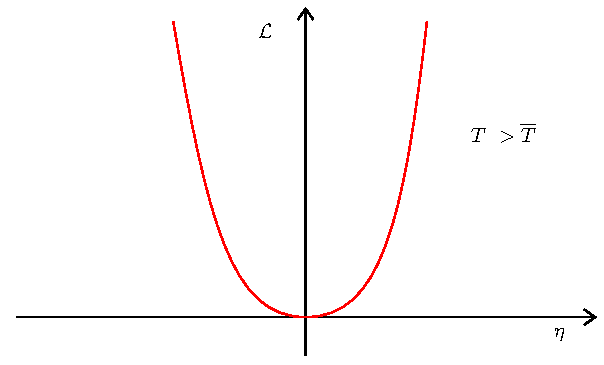
\includegraphics[width=0.8\textwidth]{./img/13__1.pdf}  \label{fig:15_10} }
\end{minipage}
\begin{minipage}[]{0.5\linewidth}
\centering
\subfloat[][Landau free energy \( \mathcal{L} \) for \( t<0 \) with \( h=0 \).]{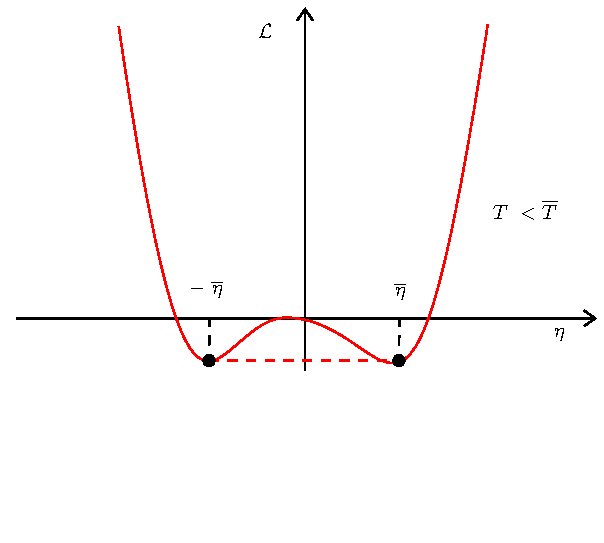
\includegraphics[width=0.8\textwidth]{./img/14__1.pdf}  \label{fig:15_11} }
\end{minipage}
\end{figure}



\section{Critical exponents in Landau's theory}
Let us therefore see what critical exponents does the Landau theory for the Ising model predict. Let us define \( t \equiv \frac{T- \bar{T} }{\bar{T} } \).

\subsubsection{Exponent \( \pmb{\beta}  \)}
This is immediately determined from what we have just seen: in fact, \( \eta \sim t^\beta  \) for \( h=0 \), \( t \rightarrow 0^- \). Since \( t<0 \), the minima of \( \mathcal{L} \) are
\begin{equation*}
  \bar{\eta } = \pm \sqrt{- \frac{at}{b}} \quad \Rightarrow  \beta = \frac{1}{2}
\end{equation*}
as expected.

\subsubsection{Exponent \( \pmb{\alpha}  \)}
The specific heat at zero field of the system is \(   C_v = - T \pdv[2]{\mathcal{L}}{T} \).
In particular, we have \( C _v \sim t^{-\alpha } \) for  \( h=0 \), \( \abs{t}  \rightarrow 0 \).
As we have seen:

\begin{itemize}
\item if \( t>0 \):  \( \mathcal{L} (\bar{\eta }=0 )= 0 \).
\item if \( t < 0 \): \( \mathcal{L}_{min} = \mathcal{L} \qty(\bar{\eta } = \pm \sqrt{- \frac{at}{b}}  ) = - \frac{a^2t^2}{4b}  \).
\end{itemize}
Hence,
\begin{equation*}
  \mathcal{L}_{min} =
    \begin{cases}
     0 & t > 0\\
     - \frac{a^2 t^2}{4b} & t < 0
    \end{cases}
\end{equation*}
Therefore:
\begin{equation*}
  c_v = - T \pdv[2]{\mathcal{L}}{T} = - T \pdv[2]{}{T} \qty(- \frac{a^2}{4b \bar{T}^2 }(T- \bar{T} )^2)
\end{equation*}
We have
\begin{equation*}
  \pdv{}{T} (\dots) \qty[- \frac{a^2}{4b \bar{T}^2 }(T- \bar{T} )^2 ] = - \frac{a^2}{2 b \bar{T}^2 } (T- \bar{T} )
\end{equation*}
\begin{equation*}
  \pdv[2]{}{T} = \pdv{}{T} \qty[ - \frac{a^2}{2 b \bar{T}^2 } (T- \bar{T} )]   = - \frac{a^2}{2 b \bar{T}^2 }
\end{equation*}
Hence, the specific heat at zero field results
\begin{equation*}
c_v =
  \begin{cases}
   0 & T > \bar{T} \\
   \frac{a^2}{2 b \bar{T}^2 } T & T < \bar{T}
  \end{cases}
\end{equation*}
We have \( t \rightarrow 0^- \) if and only if \( T \rightarrow \bar{T}^-  \), which implies \( c_v \rightarrow \frac{a^2}{2b \bar{T} } \) that is constant. Hence, in both cases:
\begin{equation*}
  \alpha =0
\end{equation*}


\subsubsection{Exponent \( \delta  \)}
Let us remind that \( h \sim \eta ^ \delta  \) at \( T = \bar{T}  \).
Considering now also an external field, the state equation of the system will be given by the differentiation of \( \mathcal{L} \):
\begin{equation*}
  \pdv{\mathcal{L}}{\eta } = a t \eta + b \eta ^3 - h = 0
\end{equation*}
Hence, the condition of equilibrium is
\begin{equation}
  h = a t \eta + b \eta ^3
  \label{eq:15_2}
\end{equation}



This tells us that, for fixed \( h \), the extreme points of \( \mathcal{L} \) are given by the values of \( \eta  \) that satisfies Eq.\eqref{eq:15_2} (see Figure \ref{fig:15_14}).

\begin{figure}[H]
\begin{minipage}[c]{0.5\linewidth}
\subfloat[][\label{fig:15_14} Plot of the Landau free energy for \( t<0 \) with an external field \( h>0 \).]{ 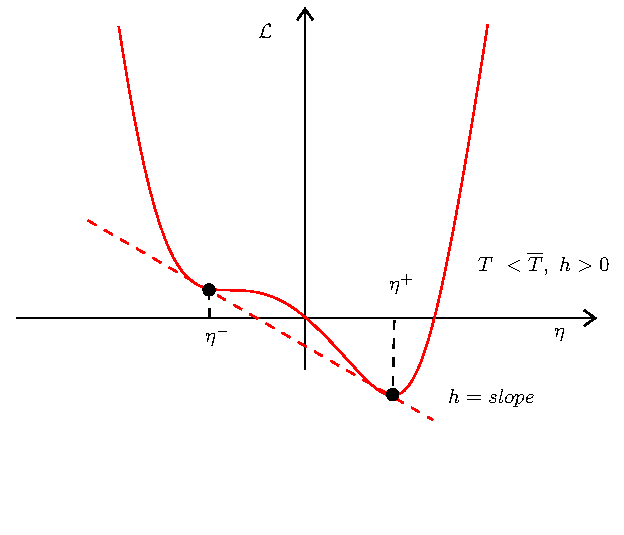
\includegraphics[width=0.8\textwidth]{./img/15__1.pdf}}
\end{minipage}
\begin{minipage}[]{0.5\linewidth}
\centering
\subfloat[][\label{fig:15_22} Plot of the Landau free energy for \( t>0 \) with an external field \( h>0 \).]{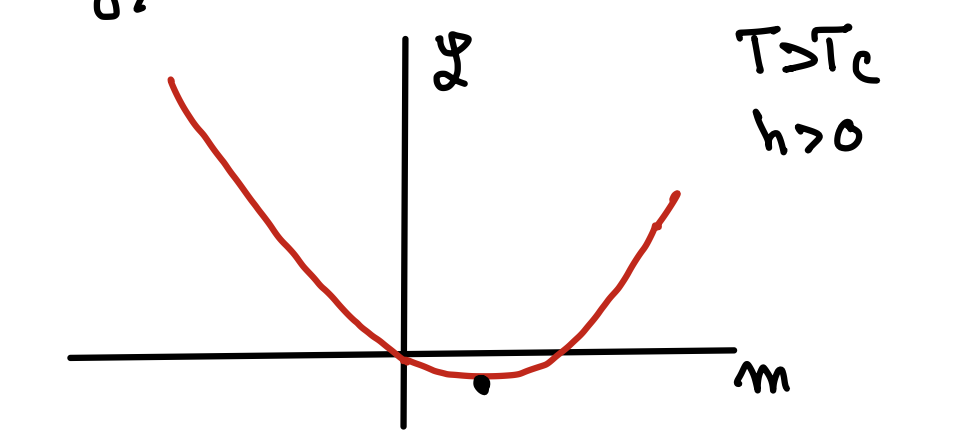
\includegraphics[width=0.8\textwidth]{./img/IMG1.png} }
\end{minipage}
\end{figure}



At the critical point \( T= \bar{T}  \) \( (t=0) \) we have \( h \sim \eta ^3 \). Therefore:
\begin{equation*}
  \delta =3
\end{equation*}


\subsubsection{Exponent \( \pmb{\gamma}   \)}
Let us remind that \( \chi _T \sim t^{- \gamma  } \) for \( h=0 \), \( \abs{t} \rightarrow 0  \).
If we now differentiate the state equation \eqref{eq:15_2} with respect to \( h \) we get:
\begin{equation*}
  a t \pdv{\eta }{h} + 3 b \eta ^2 \pdv{\eta }{h} = 1
\end{equation*}
Since \( \chi = \pdv{\eta }{h} \), we have
\begin{equation*}
  \chi = \frac{1}{at+3 b \eta ^2}
\end{equation*}
If we now set \( h=0 \), then for:
\begin{itemize}
\item \( t>0 \): we will have \( \bar{\eta } = 0  \) and thus \( \chi _T =  \frac{1}{at} \).
\item \( t<0 \): we will have \( \bar{\eta } = \pm \qty(- \frac{at}{b})^{1/2}   \) and thus \( \chi _T = - \frac{1}{2at} \).
\end{itemize}
In both cases \( \chi _T \sim  1/t \) and thus:
\begin{equation*}
  \gamma = \gamma' = 1
\end{equation*}

\subsubsection{Summary}
In summary, the Landau theory for the Ising model gives the following (mean field) values of the critical exponents
\begin{equation}
  \beta = \frac{1}{2}, \quad \alpha =0, \quad \delta =3, \quad \gamma =1
\end{equation}
which, as we expected, are identical to those we have found within Weiss mean field theory. Moreover, Landau theory does not depend on the system dimension \( d \) (as expected since is a mean field theory) but only on its symmetries.

\begin{remark}
For a \( O(n) \) (vector) model the order parameter \( \eta  \) becomes a vector field \( \va{\eta } \) with \( n \) compnents and
\begin{equation}
  \mathcal{L}_G ( \va{\eta }) = \frac{a}{2} t \va{\eta } \vdot \va{\eta } + \frac{b}{4} \qty(\va{\eta } \vdot \va{\eta } )^2 - \va{h} \vdot \va{\eta } + O \qty(\qty(\va{\eta } \vdot \va{\eta })^3 )
\end{equation}
\end{remark}


\section{First-order phase transitions in Landau theory}

As we have seen, Landau theory is based on the assumption that the order parameter is small near the critical point, and we have seen in the example of the Ising model how it can describe a continuous phase transition (in fact, for \( t \rightarrow 0 \) we have \( \eta \rightarrow 0 \)).
However, because of the symmetry properties of the Ising model we have excluded any possible cubic term; what we now want to do is to consider a more general form of
\( \mathcal{L} \) which includes also a cubic term in \( \eta  \) (in the case in which the symmetry is not violated), and see that this leads to the occurrence of a first-order phase transition.
In fact, we want to generalize to include multicritical points, or phase transitions. Let us remember that in the Ising model we have phase transition derived by symmetry breaking, while now we have another type of phase transitions.

We have seen that since the order parameter is null for \( T > \bar{T}  \) the Landau free energy cannot contain any linear term in \( \eta  \). Let us therefore consider the simplest Landau free energy that depends on a particular field:
\begin{empheq}[box=\myyellowbox]{equation}
\mathcal{L} ( \eta ,t,h)= a t \eta ^2 - w \eta ^3 + \frac{b}{2} \eta ^4 - h \eta
\label{eq:16_5}
\end{empheq}
where \( t \equiv \frac{T-T^*}{2} \) and \( w \) is an additional parameter that we fix to be positive, \( w>0 \); as in the previous case, we must have \( b>0 \) so that \( \eta  \) has finite values in the equilibrium configurations. In addiction,
\begin{equation*}
  a t = \frac{a}{2} ( T - T^*) \quad \begin{cases}
    > 0 & \text{ if } T > T^* \\
    <0 & \text{ if } T < T^*
\end{cases}
\end{equation*}
\begin{remark}
For \( w<0 \) the results are the same, but in the \( \eta <0 \) diagram.
\end{remark}
The temperature \( T^* \) is the one at which we have the continuous transition if \( w=0 \), but as we will see it doesn't have great significance now. The equilibrium configurations of the system,  will be given by:
\begin{equation*}
  \pdv{\mathcal{L}_G}{\eta } = 0 \quad \Rightarrow h = 2 a t \eta - 3 w \eta ^2 + 2b \eta ^3
\end{equation*}
In absence of external fields (\( h=0 \)), the equilibrium states becomes
\begin{equation*}
  h = 0 \quad \Rightarrow \eta ( 2 a t - 3 w \eta  + 2b \eta ^2) = 0
\end{equation*}
The solutions of this equation are
\begin{equation}
  \begin{cases}
   \bar{\eta } = 0 & \text{disordered phase}\\
  \bar{\eta_\pm } = \frac{1}{2b} \qty(3w \pm \sqrt{9 w^2 - 16abt} ) & \text{ordered phases}
  \end{cases}
\end{equation}
Let us rewrite the ordered solutions as
\begin{equation}
  \bar{\eta }_{\pm} = \frac{1}{2b} \qty(3w \pm \sqrt{9 w^2 - 16abt} ) = c \pm \sqrt{c^2 - \frac{at}{b}}
  \label{eq:16_3}
\end{equation}
with
\begin{equation*}
  c = \frac{3w}{4b}
\end{equation*}
However, these two last solutions are possible only if:
\begin{equation*}
  \bar{\eta }_{\pm} \in \R \iff c^2 - \frac{2at}{b}>0  \iff t = \frac{T-T^*}{2} < \frac{bc^2}{a} \equiv t^{**} \equiv  \frac{T^{**}-T^*}{2}
\end{equation*}
Hence, we have
\begin{equation*}
  T^{**} = T^* + \frac{2bc^2}{a} = T^* + 2t^{**}
\end{equation*}
so, since \( t^{**} \) is positive, this will occur at temperatures higher than \( T^* \).
Let us consider different cases:
\begin{itemize}
\item If \( t> t^{**} \) \( ( T > T^ {**}) \), then the system will be in the disordered phase and we have  \( \bar{\eta }_\pm \notin \R  \). The only real solution is \( \bar{\eta }=0  \) that is also the absolute minimum of \( \mathcal{L} \). The plot is shown in Figure \ref{fig:16_1}.
\begin{figure}[H]
\centering
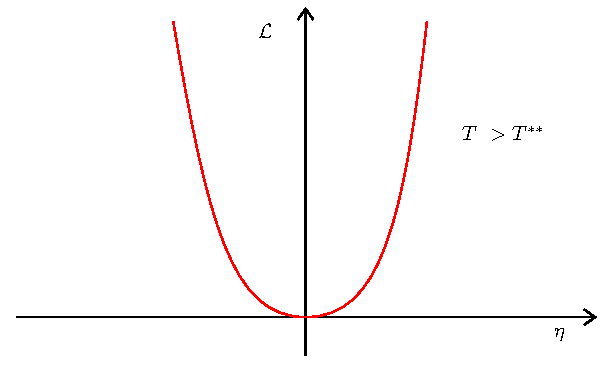
\includegraphics[width=0.6\textwidth]{./img/1.pdf}
\caption{\label{fig:16_1} Landau free energy for \( t> t^{**} \) \( ( T > T^ {**}) \). The point \( \bar{\eta }=0  \) is the absolute minimum.}
\end{figure}


\item If \( t \le t^{**} \) \( ( T \le T^ {**}) \), we have \( \bar{\eta }_\pm = c \pm \sqrt{c^2 - \frac{at}{b}} \in \R  \) are both possible solutions. One will be a local maximum and the other a local minimum.

  \begin{itemize}
  \item At \( T = T^{**}\), we have \( \bar{\eta }_- = \bar{\eta }_+   \) (flex point), as shown in Figure \ref{fig:16_2}.
  \begin{figure}[H]
  \centering
  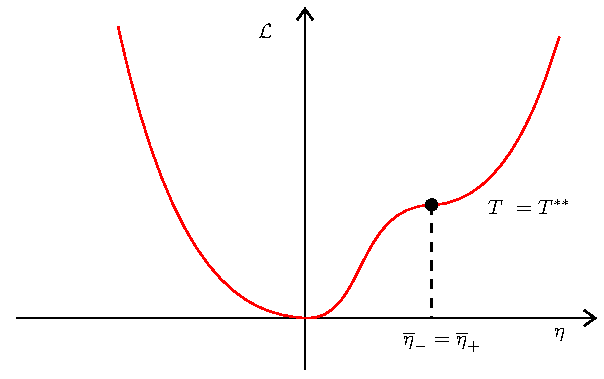
\includegraphics[width=0.6\textwidth]{./img/2.pdf}
  \caption{\label{fig:16_2} Landau free energy for \( t\le t^{**} \) \( ( T = T^ {**}) \). The point \( \bar{\eta }_- =\bar{\eta }_+   \) is a flex one.}
  \end{figure}


  \item For \( T_t < T < T^{**} \), a new minimum appears at \( \eta = \bar{\eta }_+   \), but we will have \( \mathcal{L} (\bar{\eta }_+) >0  \), so  this is only a local minimum (since \( \mathcal{L}(0)=0 \)):  in this range of temperatures the ordered phase is metastable. The plot is shown in Figure  \ref{fig:16_3}.
  \begin{figure}[H]
  \centering
  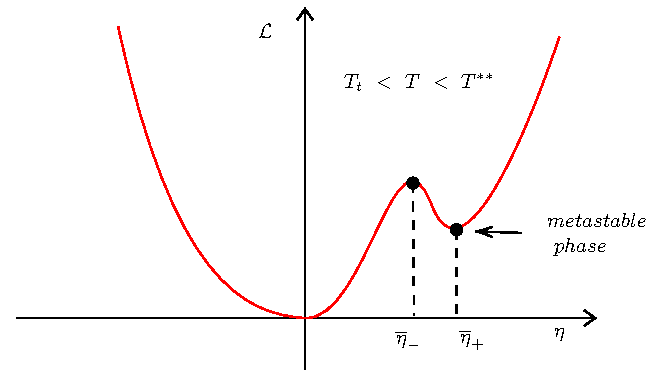
\includegraphics[width=0.6\textwidth]{./img/3.pdf}
  \caption{\label{fig:16_3} Landau free energy for \( t\le t^{**} \) \( ( T_t <T \le T^ {**}) \). The point \( \bar{\eta }_+   \) is a local minimum.}
  \end{figure}


  \item If we further decrease the temperature \( T \), we will reach a temperature \( T=T_t \) for which \(\mathcal{L} (\bar{\eta }_+ ) = 0 = \mathcal{L}(0)  \):  at this point the ordered and disordered phase coexist, so this is the temperature of a new transition! The plot is shown in Figure  \ref{fig:16_4}. \( T_t \)  is given by the coexistence condition
  \begin{equation*}
    \mathcal{L} (\bar{\eta }_+ ) = \mathcal{L} (0)
  \end{equation*}
  that is the coexistence between the disordered and ordered phases. In fact, in the plot of Figure \ref{fig:16_4} we see that there are two minima in the same line, this is  a first order transition.

  \begin{figure}[H]
  \centering
  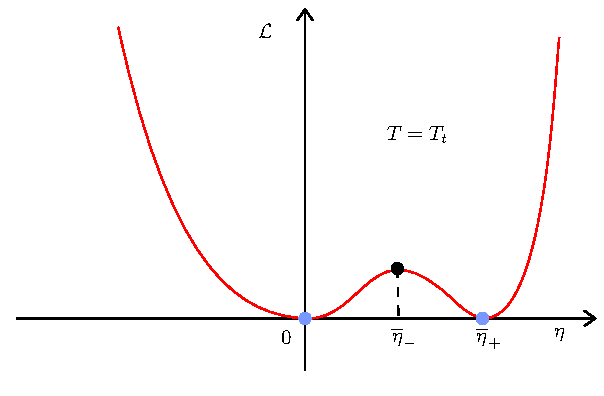
\includegraphics[width=0.6\textwidth]{./img/4.pdf}
  \caption{\label{fig:16_4} Landau free energy for \( t\le t^{**} \) \( ( T = T_t ) \). The point \( \bar{\eta }_+   \) is a minimum. The ordered and disordered phase coexist.}
  \end{figure}


  \item Finally for \( T^* < T < T_t \), \( \mathcal{\bar{\eta }_+ } \) becomes negative and so now \( \eta = \bar{\eta }_+  \) is the global minimum of \( \mathcal{L} \):  the ordered phase becomes stable and the disordered phase metastable, indeed now \( \eta =0 \) is only a local minimum (see Figure \ref{fig:16_5}).

  \begin{figure}[H]
  \centering
  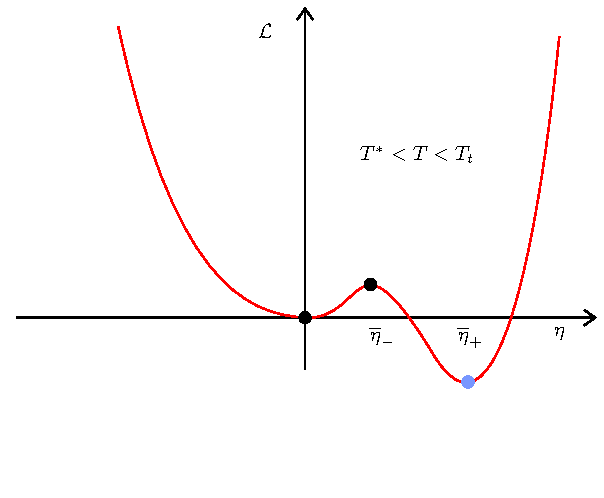
\includegraphics[width=0.6\textwidth]{./img/5.pdf}
  \caption{\label{fig:16_5} Landau free energy for \( t\le t^{**} \) \( ( T^*< T <T_t ) \). The point \( \bar{\eta }_+   \) is the global minimum.}
  \end{figure}
  \end{itemize}



Therefore, we have seen that lowering the temperature of the system, the value of \( \eta  \) for which \( \mathcal{L} \) has a global minimum changes discontinuously from \( \eta =0 \)  to \( \bar{\eta }_+  \): this is a first-order transition. All the results obtained are shown in Figure \ref{fig:16_p}.
  \begin{figure}[H]
  \begin{minipage}[c]{0.55\linewidth}
  \subfloat[][First-order transition.]{ 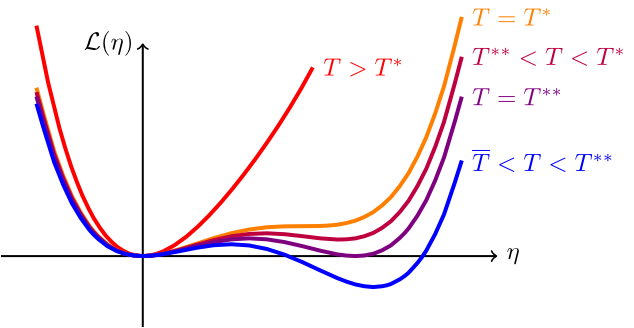
\includegraphics[width=0.8\textwidth]{./img/p_1.png}  \label{figddadada:} }
  \end{minipage}
  \begin{minipage}[]{0.55\linewidth}
  \centering
  \subfloat[][Same transition for lower values of the temperature.]{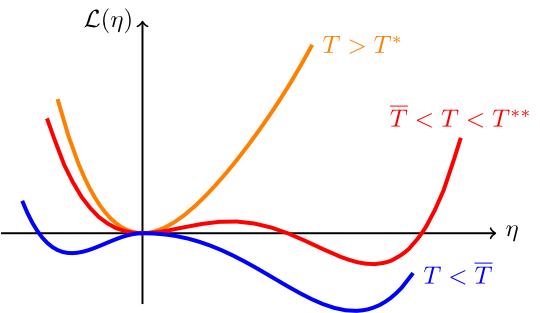
\includegraphics[width=0.8\textwidth]{./img/p_2.png}  \label{figddsds:} }
  \end{minipage}
  \caption{\label{fig:16_p} The notation in this plot is different from the one used previously. Here \( \bar{T} \equiv T^*  \), \( T^{*} \equiv T^{**} \) and \( T^{**} \equiv T_t \).  }
  \end{figure}
\end{itemize}


  As we said, at \( T=T_t \) the system undergoes a first order transition. It is defined by two conditions: it must be a minimum of \( \mathcal{L} \) and such that the value of \( \mathcal{L} \) in that minimum is zero.  Thus we can determine \( T_t \) as follows:
  \begin{equation*}
    \begin{cases}
     \pdv{\mathcal{L}}{\eta } = 0 = \eta \qty(2 a t - 3 w \eta +  b \eta ^2)  & \text{extreme condition}\\
    \mathcal{L} ( 0 ) = \mathcal{L} ( \eta _+)=0 = \eta ^2 (a t - w \eta + \frac{b}{4} \eta ^2)& \text{coexistence condition}
    \end{cases}
  \end{equation*}
  Therefore, for \( \eta \neq 0 \):
  \begin{equation*}
  \Rightarrow
    \begin{cases}
     2 a t - 3 w \eta +  b \eta ^2 = 0\\
     a t - w \eta + \frac{b}{4} \eta ^2 = 0
    \end{cases}
  \end{equation*}
  Solving with respect to \( \eta  \)  and \( t \), we get
  \begin{equation*}
    \begin{cases}
     \bar{\eta }_{t} = + \frac{w}{b} >0 \\
      t_t = \frac{w^2}{2ab} = \frac{1}{2}(T_t - T^*)}
    \end{cases}
  \end{equation*}
Since by the definition \( t = (T-T^*)/2 \), we have:
  \begin{equation}
    T_t = T^* + \frac{w^2}{ab}
  \end{equation}
  \begin{remark}
  Let us note that \( T_t >T^* \).
  \end{remark}
  Since at \( T= T_t \) there is a first order transition does the system display latent heat?
  \begin{equation*}
    s = \eval{- \pdv{\mathcal{L}}{T} }_{\eta _t} = - \frac{1}{2} a \bar{\eta }_t^2 = - \frac{a}{2} \qty(\frac{w}{b})^2
  \end{equation*}
  Hence, there is an entropy jump.
  The latent heat absorbed to go from the ordered to the disordered phase is
  \begin{equation}
    q = - T_t s = \frac{a}{2} T_t \qty(\frac{w}{b})^2
  \end{equation}




\subsection{Phase stability and behaviour of \( \pmb{\chi _T }\)}
Finally, we can also determine the susceptibility of the system:
\begin{equation*}
  \chi _T \equiv \pdv{\eta }{h}
\end{equation*}
In the presence of an external field, let us derive the equation of state with respect to \( h \):
\begin{equation*}
  \pdv{}{h} \qty(\pdv{\mathcal{L}_G}{\eta } = 0 )   = \pdv{}{h} \qty(2 a t \eta - 3 w \eta ^2 +  2b \eta ^3 = h)
\end{equation*}
Hence, since \(   \chi _T \equiv \pdv{\eta }{h} \),
\begin{equation*}
   \chi \qty(2 a t - 6 w \eta + 6 b \eta ^2 ) =1
\end{equation*}
The result is
\begin{equation}
  \chi _T = \frac{1}{2 a t - 6 w \eta + 6 b \eta ^2}
  \label{eq:16_1}
\end{equation}
We now make use of the previous equation to compute the limit of stability of the phases we have found.

\subsection{Computation of \( T^{**} \) }
As said, \( T=T^{**} \) is the value below which the ordered phase becomes a metastable state (local minima). In particular, since for \( T=T^{**} \) the point \( \bar{\eta }_-=  \bar{\eta }_+ \) is a flex point, we have the condition
\begin{equation*}
    \pdv[2]{\mathcal{L}}{\eta } = 0
\end{equation*}
thus:
\begin{equation*}
    \pdv{}{\eta } \qty(   2 a t \eta  - 6 w \eta^2 + 2b \eta ^3 = h ) = 0 \quad  \Rightarrow   2 a t - 6 w \eta + 6b \eta ^2 = \pdv{h}{\eta } =  \chi ^{-1} = 0
\end{equation*}
Remember that at \( T=T^{**} \)  the two solutions \( \bar{\eta }_\pm \) coincide, hence from Eq.\eqref{eq:16_3} we have
\begin{equation*}
  c^2 - \frac{at}{b} = 0 \quad \Rightarrow \bar{\eta }_\pm = \eta _2 = \frac{3 w}{4b}
\end{equation*}
Inserting in the expression with \( \chi ^{-1} =0 \), we have
\begin{equation*}
  \chi ^{-1} = 0 = 2 a t^{**} - 6 w \bar{\eta }_2 + 6 b \bar{\eta }_2^2
\end{equation*}
Hence,
\begin{equation}
  \iff t^{**} = \frac{9 w^2}{16 a b} = \frac{1}{2} \qty(T^{**}-T^*)
\end{equation}
Remind that for \( T_t < T < T^{**} \) the ordered phase \( \bar{\eta }_+  \) is metastable.


\subsection{Computation of \( T^* \)}
The instability of the disordered phase \( \eta =0 \) is when \( \mathcal{L} \) presents a flex point at \( \eta =0 \). Therefore, from the condition
\begin{equation*}
    \eval{\pdv[2]{\mathcal{L}}{\eta }}_{\bar{\eta } = 0 } = 0
\end{equation*}
we have
\begin{equation*}
  \chi ^{-1} = 2 a t - 6 w \eta + 6b \eta ^2 = \pdv{h}{\eta } = 0 \quad \Rightarrow
  2 a t = 0 \Rightarrow t=0
\end{equation*}
Hence, we have
\begin{equation}
\Rightarrow T = T^*
\end{equation}
thus no phase transition occurs at \( T^* \) any more. The plot of the Landau free energy in the case \( T=T^* \) is shown in Figure \ref{fig:16_6}.

\begin{figure}[H]
\centering
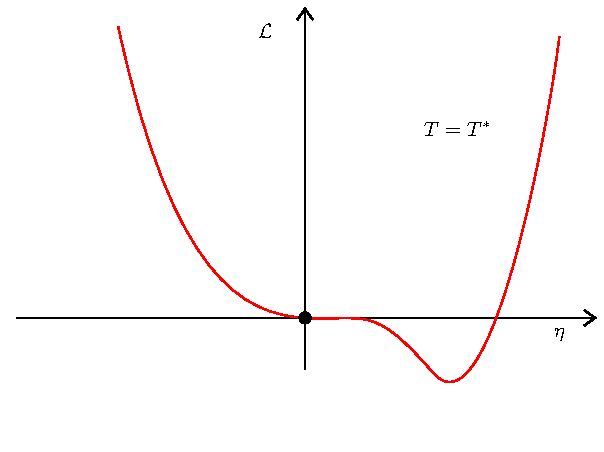
\includegraphics[width=0.6\textwidth]{./img/6.pdf}
\caption{\label{fig:16_6} Landau free energy for \( t\le t^{**} \) \( ( T =T^* ) \). The point \( \bar{\eta }_+   \) is the global minimum, while the point \( \bar{\eta }  = 0  \) is a flex point.}
\end{figure}





\section{Multicritical points in Landau theory}
It is possible for a system to have more "disarranging parameters" than the only temperature \( T \); let us call one such field \( \Delta  \). In this case the phase diagram of the system becomes richer, with coexistence and critical lines that intersect in points called multicritical points; one of the most common examples of a multicritical point is the \emph{tricritical point}, which divides a first-order transition line from a second-order one. An example of a system of the type we are considering is the Blume-Emery-Griffiths model, which we have studied in Mean field theory for the Blume-Emery-Griffiths model. In that case the additional "disarranging field" was the concentration \( x \)  of \( \text{He}^3 \), and the tricritical point is the one we called \( (x_t,T_t) \).

Such a phenomenology can be obtained within Landau theory also with terms different from a simple cubic one; in particular, we can have first order phase transitions even when the system is invariant under parity, like in the case of the Ising model. In fact in that situation we required the coefficient of \( \eta ^4 \) to be always positive, but if this is not true then \( \mathcal{L} \) will be:
\begin{equation}
  \mathcal{L} (T, \Delta, \eta ) = \frac{a (t,\Delta )}{2} \eta ^2 + \frac{b(t,\Delta )}{4} \eta ^4 + \frac{c}{6} \eta ^6 - h \eta
\end{equation}
where \( a,b \) and \( c \) are functions of two parameteres \( (T,\Delta ) \) and \( c>0 \) positive for the stability of the system (otherwise, like in the case previously considered, the minimization of \( \mathcal{L} \) leads \( \eta  \) to infinity); \( \Delta  \) is the disordered field (in the BEG model \( \Delta  \) was the \( \% \, \text{He}^3\) atoms).

\begin{remark}
To allow the coefficient of \( \eta ^4 \) to change sign, we need the \( \eta ^6 \) term.
\end{remark}



Let us study the phenomenology of \( \Delta  \) (\( \Delta _c \) is a critical value):

\begin{itemize}

\item If \( \Delta < \Delta _c \): as \( T \) decreases, \( a(T,\Delta ) \) decreases and, at \( T = T_c (\Delta ) \), becomes zero. In this region \( b(T,\Delta ) >0 \) and the system displays the standard \( (\eta ^4) \) critical point. At \( T= T_c \) we have:
\begin{equation*}
  T = T_c (\Delta ) \Rightarrow \begin{cases}
    a (T_c,\Delta ) = 0 \\
    b (T_c,\Delta ) > 0
\end{cases}
\end{equation*}

If \( a \) changes sign and  \( b \) is kept positive (which can be done varying the values of \( T \) and \( \Delta  \) in a way such that \( a \) goes to zero faster than \( b \), depending of course on their explicit expressions) then a critical transition occurs since in this case \( \eta =0 \)  becomes a local maximum for \( \mathcal{L} \), and it develops two new global minima. Therefore, the solution of the equation  \( a(T,\Delta )=0 \)  will give a line of critical points in  \( (T,\Delta ) \) plane.

\item If \( \Delta > \Delta _c \): as \( T \) decreases, \( b(T,\Delta ) \) becomes zero "before" \( a(T,\Delta ) \) and in the region $a > 0, b<0$ of the parameters a different behaviour emerges.
By imposing the conditions 
$$\frac{ \partial \mathcal{L} }{ \partial \eta } = 0; \mathcal{L}(\bar{\eta} = 0) = \mathcal{L}(\bar{\eta}_{\pm})$$
where $\bar{\eta}_{\pm}$ are the values that are not zero at which $\mathcal{L}(\bar{\eta}_{\pm})$ in a minimum (i.e. $\frac{ \partial ^2 \mathcal{L} }{ \partial \eta^{2}  }\bigg\rvert_{\bar{\eta}_{\pm}} > 0$) one can find a curve of first order phase transition given by the relation
$$a = \frac{3}{16} \frac{b^{2}}{c}\quad  \text{First order Line}$$



\begin{figure}[H]
\centering
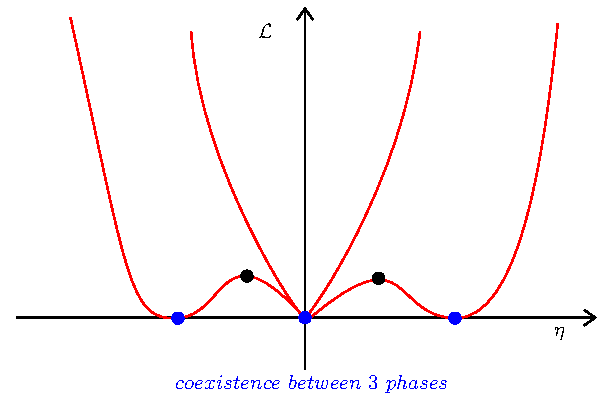
\includegraphics[width=0.6\textwidth]{./img/7.pdf}
\caption{\label{fig:16_7} Landau free energy for \( \Delta > \Delta _c \). There is coexistence between three phases, in fact there are 3 global minima.}
\end{figure}




\item Case \( \Delta = \Delta _t  \): the tricritical point is given by the values of \( \Delta = \Delta _t \)  and \( T= T_c \) such that
\begin{equation*}
  a (\Delta _t, T_t) = b (\Delta _t, T_t) = 0
\end{equation*}
 This means that when both \( a \) and \( b \) are null the system goes from exhibiting a continuous critical transition to a discontinuous first-order one; in other words, the tricritical point \( (T_{c},\Delta _{c}) \)  can be determined from the solution of the equations \( a(T,\Delta )=0 \) and \(b(T,\Delta )=0  \).

At the tricritical point the system is described by the following Landau free-energy:
\begin{equation*}
  \mathcal{L}_t = \frac{c}{6} \eta ^6
\end{equation*}
The phase diagram for $\mathcal{L}_t$ is the following:

\begin{figure}[H]
\centering
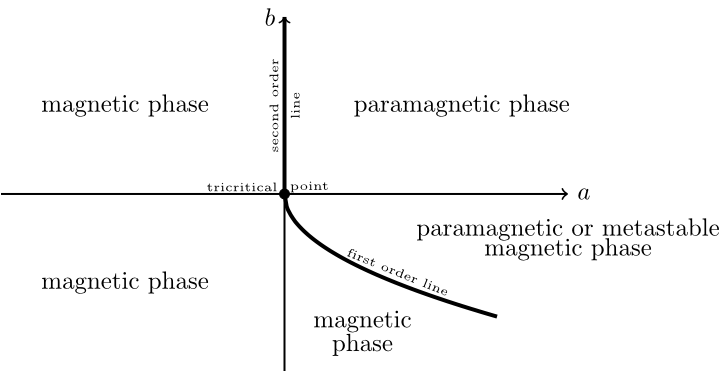
\includegraphics[width=0.8\textwidth]{./img/8.png}
\caption{\label{fig:16_8} Phase diagram of the system in  \( (a,b) \) space.}
\end{figure}


\end{itemize}

\section{Landau-deGennes theory of Liquid Crystals}
We now proceed to study a particular physical system, liquid crystals, to which we will apply Landau theory of phase transitions. As we will see the symmetries of the system will allow the Landau free energy to include a cubic term in the order parameter (which we will properly define), and so we will be able to describe the first-order transition from an isotropic to a nematic phase (which we are now going to introduce).

\subsection{What are liquid crystals?}
Liquid crystals phase (LC) can be seen as an intermediate phase between a liquid and a solid: they are liquid like any other conventional fluid, but also have internal orientational order like solid crystals. This orientational order provides them particular anisotropic properties from an optical, electric and magnetic point of view. The most common structural characteristics of the molecules that constitute liquid crystals are the following:
\begin{itemize}
\item They have an elongated, \textbf{anisotropic shape}.
\item The long axis can be approximated as a rigid backbone
\item Existence of \textbf{strong dipoles} and groups easy to polarise. 
\end{itemize}
Furthermore, it seems that the groups located at the extremities of a molecule are not relevant for the formation of phases.

 \begin{figure}[H]
 \centering
 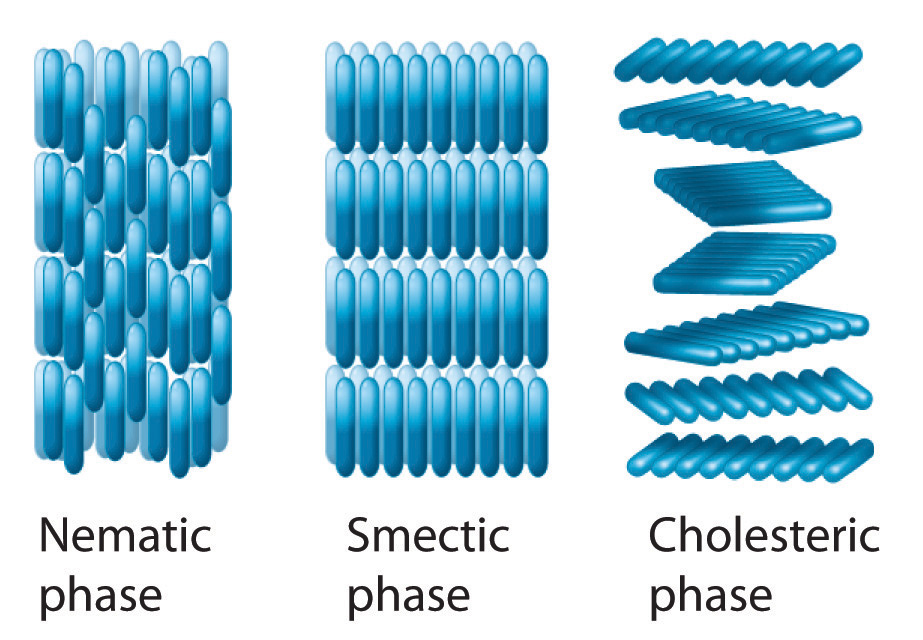
\includegraphics[width=0.6\textwidth]{./img/LC.png}
 \caption{\label{fig:16_LC} Graphical representation of the nematic, smectic and cholesteric phases of a liquid crystal.}
 \end{figure}


\noindent There is a plethora of possible liquid crystal phases; the most common are: Nematic, Cholesteric, Smectic, Columnar etc. Here we focus on the most common one, so the \textbf{Nematic Phase}.
The nematic phase is characterised by a strong and long range \textbf{orientational order}. As a measure of this order, one consider the \textbf{Director} \( \overset{\leftrightarrow}{n} (\va{r}) \). This is a 'two arrow vector' that gives the local average alignment of the elementary constituents. In this description the amplitude of \( \overset{\leftrightarrow}{n} (\va{r}) \)    is irrelevant and one takes \( \overset{\leftrightarrow}{n} (\va{r}) \) such that is unitary (i.e. \( \abs{\overset{\leftrightarrow}{n} (\va{r})}  =1 \)).
 Since there is no head-tail symmetry (apolar order), \( \overset{\leftrightarrow}{n} = -  \overset{\leftrightarrow}{n}  \) (i.e.  \(+ \overset{\leftrightarrow}{n} (\va{r}) \) and \(- \overset{\leftrightarrow}{n} (\va{r}) \) are physically equivalent).
From a optical point of view the nematic phase is \textit{birifrangent} (i.e. two refration indices, one parallel to \( \overset{\leftrightarrow}{n} (\va{r}) \) and one perpendicular (special index).

\begin{figure}[H]
\begin{minipage}[c]{0.5\linewidth}
\subfloat[][Isotropic phase.]{ 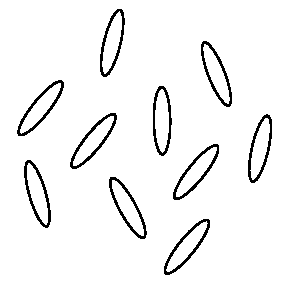
\includegraphics[width=0.8\textwidth]{./img/9.pdf}  \label{fig:16_9_1} }
\end{minipage}
\begin{minipage}[]{0.5\linewidth}
\centering
\subfloat[][Nematic phase.]{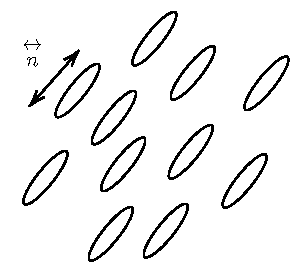
\includegraphics[width=0.8\textwidth]{./img/10.pdf}  \label{fig:16_9_2} }
\end{minipage}
\label{fig:16_9}
\end{figure}



\subsection{Definition of an order parameter for nematic liquid crystals}
What we now want to do is to apply Landau theory to liquid crystals in order to study the transition from an isotropic to a nematic phase (Figure \ref{fig:16_9}); therefore, we must define an order parameter for such a system. This is absolutely not trivial, and there are two ways to do it a microscopic and a macroscopic one. We will use a macroscopic approach.

\subsubsection{Macroscopic approach}
From a macroscopic point of view we have already stated that an important difference between the disordered and nematic phases consists in the response functions when the liquid crystal is subjected to magnetic or electrical fields. Hence, a macroscopic definition of an order parameter for LC phase is based on the system response when subject to fields. For instance, supposing that we have a liquid crystal subject to an external magnetic field \( \va{H} \), the diamagnetic response of the system will be measurable in terms of its magnetization \( \va{M} \), and in particular:
\begin{equation}
  \va{M} = \bar{\bar{\chi } } \va{H}
\end{equation}
where  \(  \bar{\bar{\chi } } \) is the response function matrix, namely the magnetic susceptibility of the system. In components we have:
\begin{equation}
  M_ \alpha = \chi _{\alpha \beta } H _{\beta }
\end{equation}
where the inexes \( \alpha , \beta  \) stands for \( x,y,z \). If \( \va{H} \) is static, then \( \chi  \) is symmetric, i.e.
\begin{equation*}
  \chi _{\alpha \beta } = \chi _{\beta \alpha }
\end{equation*}
In the isotropic phase \( \chi  \) will also be diagonal, namely
\begin{equation*}
  \chi _{\alpha \beta } = \chi  \delta _{\alpha \beta }
\end{equation*}
while in the nematic phase
For a LC in the neumatic one has
\begin{equation}
  \chi _{\alpha \beta } =
  \begin{pmatrix}
  \chi _\bot   &  0 & 0 \\
    0 &  \chi _ \bot & 0 \\
    0 &  0 &  \chi _\parallel
  \end{pmatrix}
\end{equation}
where, as before, we have supposed that the director \( \overset{\leftrightarrow}{n} \) is parallel to the \( z \) direction.

Therefore we could build an order parameter in terms of the susceptibility \( \chi  \), and this parameter will necessarily have a tensorial nature (since \( \chi  \) itself is in general a tensor), so it will not be a simple scalar like in the previous case. Since we want our order parameter to vanish in the disordered phase, we can define it "removing" from \( \chi  \) its isotropic component. In other words, in components we can define:
\begin{equation}
  Q_{\alpha \beta } = A \qty(\chi _{\alpha \beta } - \frac{1}{3} \delta _{\alpha \beta }\Tr \bar{\bar{\chi } }  )
\end{equation}
where \( A \) is a constant. In this way \( Q \) is a good tensorial order parameter. In particular, the order parameter is a second rank traceless tensor. Let us note that its definition is completely general, and in fact it is useful also to describe other kinds of phases, not only the uniaxial nematic one.

 It is possible to show that \(   Q_{\alpha \beta }  \) can be written in terms of the local average orientiational order of the elementary constituents, \(  \overset{\leftrightarrow}{n} (\va{r}) \) and the degree of local order given by a scalar \( S(\va{r}) \). Hence, we can define
\begin{equation}
  Q_{\alpha \beta } (\va{r}) = S (\va{r}) \qty(n_{\alpha } (\va{r}) n_{\beta } (\va{r}) - \frac{1}{3}\delta _{\alpha \beta })
\end{equation}
The advantage of this definition of the order parameter (which is the one we will use in the following) is that it also takes into account the degree of orientation and the mean direction.
By definition \( Q \) is symmetric and traceless\footnote{A matrix whose trace is zero is said to be traceless.}, so in general way we can write it as:
\begin{equation}
  Q  =
  \begin{pmatrix}
  q_1   & q_2  & q_3 \\
  q_2   & q_4  & q_5 \\
  q_3   & q_5  & -q_1-q_4
  \end{pmatrix}
\end{equation}



\subsection{Landau-de Gennes theory for nematic liquid crystals}
Since we now have a proper order parameter, we can formulate the Landau theory for the phase transitions of nematic liquid crystals (also called Landau-de Gennes theory). In particular we want to study the transition between the isotropic and nematic phase, and we call \( T_{n-i} \) the temperature at which it occurs.

As we have already stated, the Landau free energy \( \mathcal{L} \)  must be consistent with the symmetries of the system, so in this case it must be invariant under rotations. Now, since \( Q \) transforms as a tensor under rotations and \( \mathcal{L} \) must be a scalar, it will contain terms of the form  \( \Tr \bar{\bar{Q} }^P \); to the fourth order we will have (the linear term is absent because by definition \( Q \) is traceless, i.e. \( \Tr(Q) = 0  \)):
\begin{equation*}
  \mathcal{L} = \mathcal{L}_0 + \frac{1}{2} A(T) \Tr \bar{\bar{Q} }^2 + \frac{1}{3} B(T) \Tr \bar{\bar{Q} }^3 + \frac{1}{4} C(T) \qty[ \qty(\Tr \bar{\bar{Q} }^2  )^2 + \Tr \bar{\bar{Q} }^4 ]
\end{equation*}

In reality this expression, and in particular the quartic term, can be simplified: in fact it is a property (which we will not prove) of any \( n \times n \)  symmetric matrix that \( \Tr \bar{\bar{Q} }^s \) with \( s>n \)  can be expressed as a
 polynomial of \( \Tr \bar{\bar{Q} }^p \) with \( p<n \), so in our case any \( \Tr \bar{\bar{Q} }^s \) with \( s\geq 4 \) can be expressed in terms of \( \Tr \bar{\bar{Q} }^2 \) and \( \Tr \bar{\bar{Q} }^3 \) (we are automatically neglecting  \( \Tr \bar{\bar{Q} } \)  since in our case it vanishes, but in general it must be considered).
 Therefore, we can write the Landau free energy as:
 \begin{equation}
   \mathcal{L} = \mathcal{L}_0 + \frac{1}{2} A(T) \Tr \bar{\bar{Q} }^2 + \frac{1}{3} B(T) \Tr \bar{\bar{Q} }^3 + \frac{1}{4} C(T)  \qty(\Tr \bar{\bar{Q} }^2  )^2
 \end{equation}
or, in components:
\begin{equation}
  \mathcal{L} = \mathcal{L}_0 + \frac{1}{2} A(T) Q_{\alpha \beta }Q_{\beta \alpha } + \frac{1}{3} B(T) Q_{\alpha \beta } Q_{\beta \gamma  } Q_{\gamma  \alpha }+ \frac{1}{4} C(T) \qty(Q_{\alpha \beta } Q_{\beta  \alpha })^2
\end{equation}

\begin{remark}
Since each \( 3 \times 3 \) matrix satisfies the relation
\begin{equation*}
   \Tr \bar{\bar{Q} }^4 = \frac{1}{2} \qty( \Tr \bar{\bar{Q} }^2)^2
\end{equation*}
the term proportional to \( C(T) \) can be written as \( \frac{1}{2}C(T)  \Tr \bar{\bar{Q} }^4 \).
\end{remark}

Let us note that since our order parameter is a tensor its invariance under rotations does not exclude the possible existence of terms with odd powers of \( Q \) in \( \mathcal{L} \), in particular the cubic one.


For the most general case of a \emph{biaxial}  nematic phase \( \bar{\bar{Q} }  \) can be diagonalized giving
\begin{equation}
  Q_{\alpha \beta } =
  \begin{pmatrix}
  \frac{2}{3}S   & 0  & 0 \\
    0 &  - \frac{1}{3} \qty(S+ \eta  ) & 0 \\
    0 &  0 & - \frac{1}{3}\qty(S- \eta  )
  \end{pmatrix}
\end{equation}
where we remind that \( S \) is the degree of local order.
If \( \eta = 0 \) we have the standard \emph{uniaxial} nematic phase and the order parameter becomes
\begin{equation}
  Q_{\alpha \beta } =
  \begin{pmatrix}
  \frac{2}{3}S   & 0  & 0 \\
    0 &  - \frac{1}{3}S & 0 \\
    0 &  0 & - \frac{1}{3}S
  \end{pmatrix}
  \label{eq:16_4}
\end{equation}

Now, from the expression of \( Q \) in the case of a uniaxial nematic liquid crystal we have:
\begin{equation*}
 \Tr \bar{\bar{Q} }^2  = \frac{2}{3} S^2, \quad \Tr \bar{\bar{Q} }^3  = \frac{2}{9} S^3, \quad \qty(\Tr \bar{\bar{Q} }^2)^2  = \frac{4}{9} S^4
\end{equation*}
Hence, for uniaxial nematic liquid crystal the Landau free energy becomes
\begin{equation}
  \mathcal{L} = \mathcal{L}_0 +  \frac{A(T)} {3}S^2 + \frac{2}{27} B(T) S^3 + \frac{C(T)}{9}  S^4
\end{equation}
so that, supposing that \( B \) and \( C \) do not depend on the temperature (i.e. \( B(T) =B \) and \( C(T) = C \)), while  \( A(T) \simeq A (T-T^*) \), we have:
\begin{equation}
  \mathcal{L} = \mathcal{L}_0 + \frac{A}{3} (T-T^*) S^2 + \frac{2}{27} B S^3 + \frac{C}{9} S^4
\end{equation}
This Landau free energy has exactly the same form of the one we studied in first-order phase transitions in Landau theory, with the substitutions:
\begin{equation*}
  a = \frac{2}{3} A, \quad w = -\frac{2}{27} B, \quad b = \frac{2}{9} C
\end{equation*}
Applying the results we have already found we will have that the first-order transitions between the isotropic and nematic phases occurs at the temperature:
\begin{equation}
  T_{t} =  T^* + \frac{w^2}{ba}=  T^* + \frac{B^2}{27 A C}
\end{equation}






\end{document}